\chapter{One Sample Confidence Intervals on a Mean When the Population Variance is Known}
\section{Key Concepts and Definitions}

\begin{definitionbox}{Key Terms}
\textbf{Population:} A group of interest (typically large). \\
\vspace{0.2em}

\textbf{Sample:} A subset of a population. \\

\textbf{Parameter (of population):} A numerical characteristic of a population. These are usually \textcolor{blue}{unknown} in real-life settings. \\
\hspace*{1em} $\mu$: population mean \\
\hspace*{1em} $\sigma^2$: population variance \\
\hspace*{1em} $\sigma$: population standard deviation \\
\textcolor{blue}{Note: Different from a parameter of a distribution.} \\

\textbf{Statistic (of sample):} A numerical characteristic of a sample, which is calculated and known (i.e., a function of the data). \\
\hspace*{1em} $\bar{x}$: sample mean \\
\hspace*{1em} $s^2$: sample variance \\
\hspace*{1em} $s$: sample standard deviation\\
\vspace{0.2em}

\textbf{Statistical Inference:} Use statistics (known) to make conclusions on parameters (unknown) and quantify the degree of certainty of statements made.

\end{definitionbox}
\noindent
The sample mean, $\bar{x} = \frac{1}{n} \sum_{i=1}^{n} x_i$, is a number we use to estimate the population mean, $\mu$. This is called a \textbf{point estimate}. % one value, single best estimate of a parameter

\vspace{1em}

But, we know it’s not equal to $\mu$. Then, we’d rather estimate the population mean using an \textbf{interval estimate} that gives a \textit{range of real numbers} that we hope contains the population mean, $\mu$.
\vspace{2em}
\textcolor{orange!80!black}{\section*{Examples}}

\begin{itemize}
    \item $\bar{x}$ is a point estimate of $\mu$
    \item $s^2$ is a point estimate of $\sigma^2$
    \item $s$ is a point estimate of $\sigma$
\end{itemize}

\vspace{0.5em}
\textcolor{blue}{\textit{(All calculated with data from a sample)}}

\vspace{1.5em}

Due to the nature of randomness and calculating based on a subset, statistics are not guaranteed to be exactly equal to parameters.

\vspace{1em}

Therefore, we create \underline{intervals} around statistics which we believe capture the parameter.

\vspace{2em}

\noindent
\textbf{Confidence Interval:} A range of values we believe captures a parameter with a certain level of confidence.

\vspace{1em}

\begin{center}
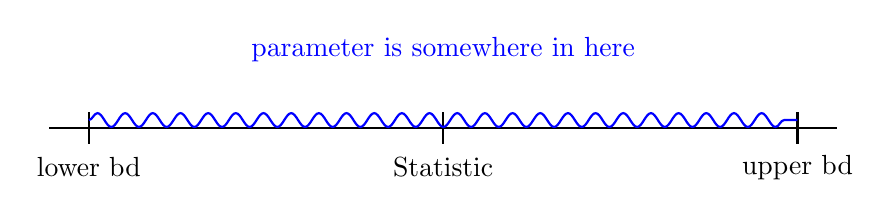
\begin{tikzpicture}
    \draw[thick] (-5,0) -- (5,0);
    \draw[thick] (-4.5,0.2) -- (-4.5,-0.2); % lower bd
    \draw[thick] (0,0.2) -- (0,-0.2);       % statistic
    \draw[thick] (4.5,0.2) -- (4.5,-0.2);   % upper bd
    \node at (-4.5,-0.5) {lower bd};
    \node at (0,-0.5) {Statistic};
    \node at (4.5,-0.5) {upper bd};
    \node[blue] at (0,1) {parameter is somewhere in here};
    \draw[blue, thick, decorate, decoration={snake}] (-4.5,0.1) -- (4.5,0.1);
\end{tikzpicture}
\end{center}

\vspace{2em}

\noindent
\textbf{Skeleton (general form):}
\[
\text{Estimator (statistic)} \pm \left( \text{value from a reference distribution} \times \text{standard error of estimate} \right)
\]

\vspace{0.5em}
\textcolor{blue}{\textit{Z or t} \hspace{1em} \textit{Standard error = std. dev. of sampling distribution}}

\vspace{1em}
The exact form depends on the parameter of interest and the information available.

\vspace{2em}

\textbf{Interpretation of CI’s:}

Suppose we construct a $C\%$ confidence interval.

\vspace{0.5em}
\textbf{Intuitive Interpretation:} We are $C\%$ confident the target parameter is inside the CI constructed.

\vspace{0.5em}
\textbf{Formal Definition:} In repeated sampling, approximately $C\%$ out of all the $C\%$ CI’s constructed captures the parameter.

\vspace{1em}
(See Slide 11)

\vspace{2em}

\begin{center}
% \includegraphics[width=0.85\textwidth]{ci_visual.png}
\begin{center}
\fbox{\parbox{0.8\textwidth}{
\centering
[Insert visual showing 95\% confidence intervals for $\mu$ -- see slide image with intervals]}
}
\end{center}

\end{center}

\vspace{0.5em}
Approximately 95\% of the 1000 intervals (i.e., approx. 950) capture $\mu$.
\section{Confidence Interval for $\mu$ (Known Variance)}

Let $X_1, X_2, ..., X_n$ be iid $N(\mu, \sigma^2)$, where $\mu$ is unknown and $\sigma$ is known.

We know that:
\[
Z = \frac{\bar{X} - \mu}{\sigma / \sqrt{n}} \sim N(0, 1)
\]
and
\[
P(-1.96 < Z < 1.96) = 0.95
\]
Therefore:
\[
P\left( -1.96 < \frac{\bar{X} - \mu}{\sigma / \sqrt{n}} < 1.96 \right) = 0.95
\Rightarrow P\left( \bar{X} - 1.96 \frac{\sigma}{\sqrt{n}} < \mu < \bar{X} + 1.96 \frac{\sigma}{\sqrt{n}} \right) = 0.95
\]

\vspace{1.5em}
\textbf{Interpretation of Confidence Interval:}

\begin{itemize}
  \item This is a random interval $\bar{X} \pm 1.96 \frac{\sigma}{\sqrt{n}}$
  \item The interval is random since $\bar{X}$ is random due to sampling.
  \item The population mean $\mu$ is a fixed, but unknown, number.
  \item The probability $\mu$ is inside the random interval is 0.95 (success rate of the method).
  \item 95\% of all samples give an interval that captures $\mu$, and 5\% do not.
\end{itemize}

\vspace{1em}
Once we observe our sample:

\begin{itemize}
  \item This is \textbf{not} a random interval $\bar{X} \pm 1.96 \frac{\sigma}{\sqrt{n}}$
  \item The probability $\mu$ is inside this interval is either 1 or 0
\end{itemize}

\vspace{1em}
\textbf{Confidence Interval Isn’t Always Right:}

Not all CIs contain the true value of the parameter. This can be illustrated by plotting many intervals simultaneously and observing.

---

\vspace{2em}
\textcolor{gray}{\textbf{R Output:}}

\begin{lstlisting}[language=R]
## Step 1. Generate random samples;
set.seed(2017)
m = 50;       # m = number of samples;
n = 25;       # n = number of obs in sample;
mu.i = 0;     # mu.i = mean of obs;
sigma.i = 5;  # sigma.i = std. dev. of obs;

mu.total = n * mu.i;          # mean of Total;
sigma.total = sqrt(n) * sigma.i;  # std. dev. of Total;
\end{lstlisting}

\vspace{1em}
\textcolor{gray}{\textbf{R Output:}}

\begin{lstlisting}[language=R]
## Step 2. Construct CIs;
xbar = rnorm(m, mu.total, sigma.total) / n;
SE = sigma.i / sqrt(n);

alpha = 0.10;
z.star = qnorm(1 - alpha / 2);
\end{lstlisting}

\vspace{1em}
\textcolor{gray}{\textbf{R Output:}}

\begin{lstlisting}[language=R]
## Step 3. Graph CIs;
matplot(rbind(xbar - z.star * SE, xbar + z.star * SE),
        rbind(1:m, 1:m),
        type = "l", lty = 1,
        xlab = " ", ylab = " ");
abline(v = 0, lty = 2);
\end{lstlisting}
\vspace{2em}
Image for Slide 11 will be inserted here.

\vspace{2em}

\section*{Confidence Interval for the Mean of a Normal Population}

Draw an SRS (Simple Random Sample) of size $n$ from a Normal population having unknown mean $\mu$ and \textbf{known} standard deviation $\sigma$. A level $C$ confidence interval for $\mu$ is:

\[
\bar{x} \pm z_{\ast} \cdot \frac{\sigma}{\sqrt{n}}
\]

The critical value $z_{\ast}$ is illustrated in a Figure below and depends on $C$.

\vspace{2em}
Image for Slide 13 will be inserted here.
\section*{Large Sample CI for $\mu$ (Normal data)}

\[
\bar{x} \pm z_{\alpha/2} \cdot \frac{\sigma}{\sqrt{n}}
\]

Valid if:
\begin{itemize}
  \item $n$ large
  \item random sample from a Normal distribution
  \item independent observations
\end{itemize}

Some definitions:
\begin{itemize}
  \item $1 - \alpha$ is the confidence coefficient
  \item $100(1 - \alpha)\%$ is the confidence level
\end{itemize}


\section*{One Sample CI on the Population Mean $\mu$}

\begin{itemize}
  \item When population standard deviation $\sigma$ is \textbf{known}
  \item Formula: $\bar{x} \pm z_{\alpha/2} \cdot \frac{\sigma}{\sqrt{n}}$
  \item Margin of error comes from standard normal and standard error
\end{itemize}

How to find $z_{\alpha/2}$?

Example: Find $z_{\alpha/2}$ for a 95\% CI on $\mu$:
\[
1 - \alpha = 0.95, \quad \alpha = 0.05, \quad \alpha/2 = 0.025
\]
\[
z_{\alpha/2} = 1.96 \quad (\text{from table or R: } \texttt{qnorm(0.975)})
\]


\section*{Table of Common $z$-values}

\begin{center}
\begin{tabular}{|c|c|c|}
\hline
Confidence coefficient & Confidence level & $z$ \\
\hline
0.90 & 90\% & 1.645 \\
0.95 & 95\% & 1.96 \\
0.99 & 99\% & 2.576 \\
\hline
\end{tabular}
\end{center}



\section*{Example}

Playbill magazine reported that the mean annual household income of its readers is \$119{,}155. Assume this estimate is based on a sample of 80 households, and that the population standard deviation is known to be $\sigma = 30{,}000$.

\begin{itemize}
  \item $\bar{x} = 119{,}155$
  \item $n = 80$
  \item $\sigma = 30{,}000$
\end{itemize}

\textbf{Tasks:}
\begin{enumerate}
  \item[(a)] Develop a 90\% confidence interval estimate of the population mean.
  \item[(b)] Develop a 95\% confidence interval estimate of the population mean.
  \item[(c)] Develop a 99\% confidence interval estimate of the population mean.
\end{enumerate}



\textbf{90\% CI Calculation}

\[
\bar{x} \pm z_{\alpha/2} \cdot \frac{\sigma}{\sqrt{n}} = 119{,}155 \pm 1.645 \cdot \frac{30{,}000}{\sqrt{80}}
\]
\[
= 119{,}155 \pm 5{,}500.73
\]
\[
= (113{,}654.27, \; 124{,}655.73)
\]

\textbf{95\% CI Calculation}

\[
\bar{x} \pm z_{\alpha/2} \cdot \frac{\sigma}{\sqrt{n}} = 119{,}155 \pm 1.96 \cdot \frac{30{,}000}{\sqrt{80}}
\]
\[
= 119{,}155 \pm 6{,}574.04
\]
\[
= (112{,}580.96, \; 125{,}729.04)
\]


\textbf{99\% CI Calculation}

\[
\bar{x} \pm z_{\alpha/2} \cdot \frac{\sigma}{\sqrt{n}} = 119{,}155 \pm 2.576 \cdot \frac{30{,}000}{\sqrt{80}}
\]
\[
= 119{,}155 \pm 8{,}620.04
\]
\[
= (110{,}534.96, \; 127{,}775.04)
\]


\textbf{Interpretation}


We are 99\% confident the mean household income of magazine readers is between \$110{,}534.96 and \$127{,}775.04.

\section*{Example: Estimating Mean Number of Cars Sold}

\vspace{1em}

\noindent\textbf{Scenario:}

\vspace{0.5em}

The number of cars sold annually by used car salespeople is known to be \textbf{normally distributed}, with a population standard deviation of $\sigma = 15$. A random sample of $n = 15$ salespeople was taken, and the number of cars each sold is recorded below. Construct a \textbf{95\% confidence interval} for the population mean number of cars sold, and provide an interpretation.

\vspace{1em}

\noindent\textbf{Raw data:}

\[
\begin{matrix}
79 & 43 & 58 & 66 & 101 \\
63 & 79 & 33 & 58 & 71 \\
60 & 101 & 74 & 55 & 88 \\
\end{matrix}
\]

\vspace{0.5em}

\noindent The sample mean is:

\[
\bar{x} = \frac{79 + 43 + \cdots + 55 + 88}{15} = 68.6
\]

\vspace{1em}

\noindent\textbf{R function:}

\begin{tcolorbox}[colback=gray!10, colframe=gray!50, arc=2mm]
\begin{verbatim}
simple.z.test = function(x, sigma, conf.level = 0.95) {
  n = length(x);
  xbar = mean(x);
  alpha = 1 - conf.level;
  zstar = qnorm(1 - alpha/2);
  SE = sigma / sqrt(n);
  xbar + c(-zstar * SE, zstar * SE);
}
\end{verbatim}
\end{tcolorbox}

\vspace{0.5em}

\noindent\textbf{R output:}

\begin{tcolorbox}[colback=gray!10, colframe=gray!50, arc=2mm]
\begin{verbatim}
# Step 1. Entering data;
cars = c(79, 43, 58, 66, 101, 63, 79,
         33, 58, 71, 60, 101, 74, 55, 88)

# Step 2. Finding CI;
simple.z.test(cars, 15)

## [1] 61.00909 76.19091
\end{verbatim}
\end{tcolorbox}

\vspace{1em}

\noindent\textbf{Interpretation:} \textbf{We estimate that the mean number of cars sold annually by all used car salespeople lies between 61 and 76, approximately. This type of estimate is correct 95\% of the time.}

\vspace{1em}

\begin{tcolorbox}[colback=blue!5!white, colframe=blue!75!black,
  title=\textbf{Cases Where Valid}, fonttitle=\bfseries,
  coltitle=white, colbacktitle=blue!90!black, arc=2mm]

\begin{itemize}
  \item Large samples where population is \textbf{normal}.
  \item Large samples where population is \textbf{not normal} (By CLT).
  \item Small samples where population is \textbf{normal}.
\end{itemize}

\textit{Note: A sample is considered large if $n \geq 30$.}
\end{tcolorbox}

\textbf{Example.} Suppose a student measuring the boiling temperature of a certain liquid observes the readings (in degrees Celsius) 102.5, 101.7, 103.1, 100.9, 100.5, and 102.2 on 6 different samples of the liquid. He calculates the sample mean to be 101.82. If he knows that the distribution of boiling points is Normal, with standard deviation 1.2 degrees, what is the confidence interval for the population mean at a 95\% confidence level?\\
\textbf{A confidence interval} uses sample data to estimate an unknown population parameter with an indication of how accurate the estimate is and of how confident we are that the result is correct.

\vspace{1em}

The \textbf{interval} often has the form\\
\hspace*{2em}estimate $\pm$ margin of error

\vspace{1em}

The \textbf{confidence level} is the success rate of the method that produces the interval.
 A level $C$ \textbf{confidence interval for the mean} $\mu$ of a Normal population with \textbf{known} standard deviation $\sigma$, based on an SRS of size $n$, is given by
\[
\bar{x} \pm z^\star \frac{\sigma}{\sqrt{n}}
\]

The \textbf{critical value} $z^\star$ is chosen so that the standard Normal curve has area $C$ between $-z^\star$ and $z^\star$. \\

Other things being equal, the \textbf{margin of error} of a confidence interval gets smaller as
\begin{itemize}
    \item the confidence level $C$ decreases,
    \item the population standard deviation $\sigma$ decreases, and
    \item the sample size $n$ increases.
\end{itemize}
\vspace{\baselineskip} 
\section{APPENDIX}


Interval estimators are commonly called \textbf{confidence intervals}. The upper and lower endpoints of a confidence interval are called the \textbf{upper} and \textbf{lower confidence limits}, respectively. The probability that a (random) confidence interval will enclose $\theta$ (a fixed quantity) is called the \textbf{confidence coefficient}.\\


Suppose that $\hat{\theta}_L$ and $\hat{\theta}_U$ are the (random) lower and upper confidence limits, respectively, for a parameter $\theta$. Then, if
$$P(\hat{\theta}_L \leq \theta \leq \hat{\theta}_U) = 1 - \alpha,$$
the probability $(1 - \alpha)$ is the \textbf{confidence coefficient}.

\subsection*{Pivotal quantities}
One very useful method for finding confidence intervals is called the \textbf{pivotal method}. This method depends on finding a pivotal quantity that possesses two characteristics:
\begin{itemize}
    \item It is a function of the sample measurements and the unknown parameter $\theta$, where $\theta$ is the \textbf{only} unknown quantity.
    \item Its probability distribution does not depend on the parameter $\theta$.
\end{itemize}


